\begin{figure}
\centering
    \begin{subfigure}{.24\textwidth}
        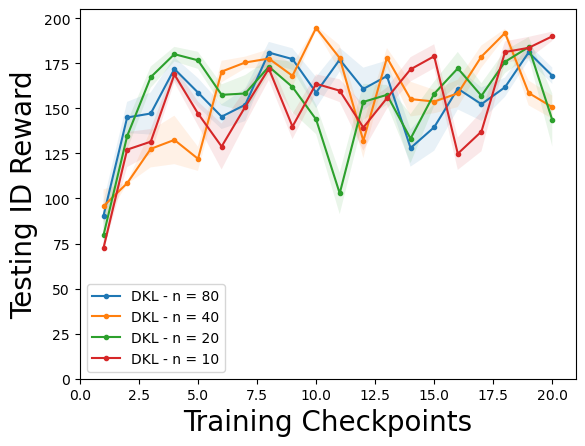
\includegraphics[width=\textwidth]{sections/011_icml2022/resources/CartPole-v0-mean_reward_-testing-hyperparameter-n_inducing_points-dkl.png}  
    \end{subfigure}
        \begin{subfigure}{.24\textwidth}
        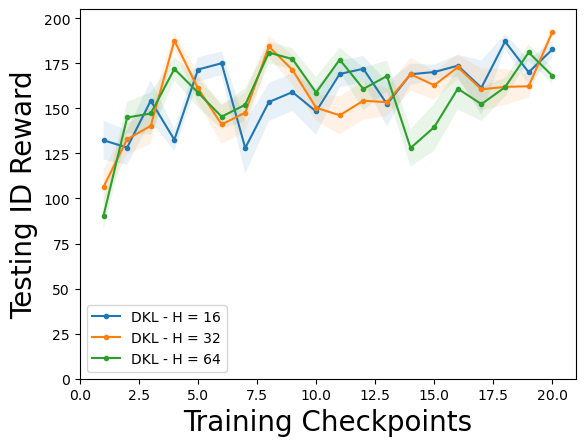
\includegraphics[width=\textwidth]{sections/011_icml2022/resources/CartPole-v0-mean_reward_-testing-hyperparameter-latent_dim-dkl.png}  
    \end{subfigure}
        \begin{subfigure}{.24\textwidth}
        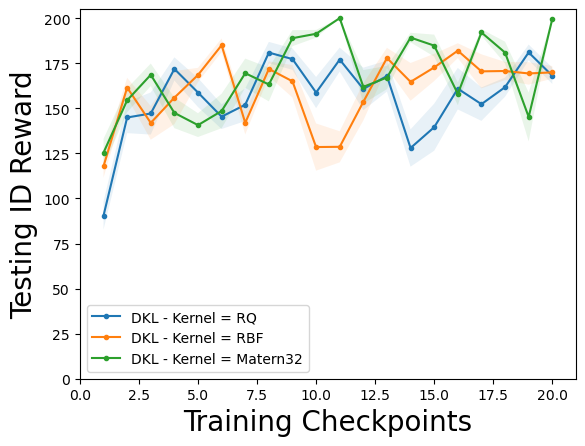
\includegraphics[width=\textwidth]{sections/011_icml2022/resources/CartPole-v0-mean_reward_-testing-hyperparameter-kernel-dkl.png}  
    \end{subfigure}
        \begin{subfigure}{.24\textwidth}
        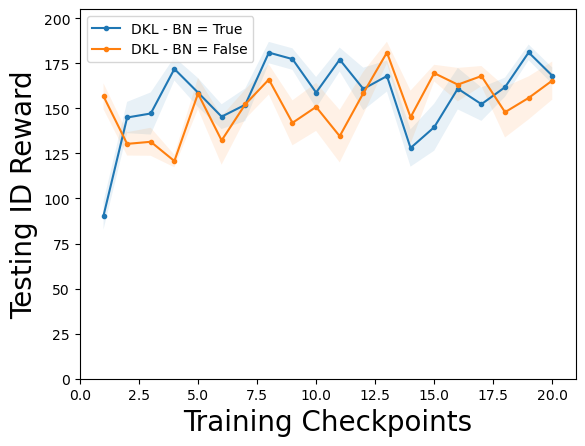
\includegraphics[width=\textwidth]{sections/011_icml2022/resources/CartPole-v0-mean_reward_-testing-hyperparameter-bn-dkl.png}  
    \end{subfigure}
    
    \begin{subfigure}{.24\textwidth}
        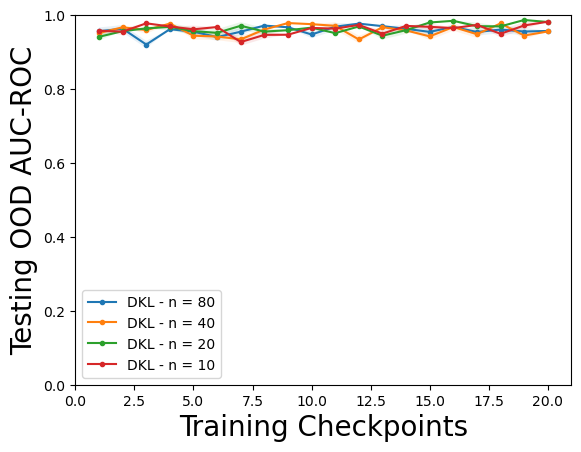
\includegraphics[width=\textwidth]{sections/011_icml2022/resources/CartPoleOOD-v0-AUC-ROC-epistemic_-testing-hyperparameter-n_inducing_points-dkl.png}
    \end{subfigure}
        \begin{subfigure}{.24\textwidth}
        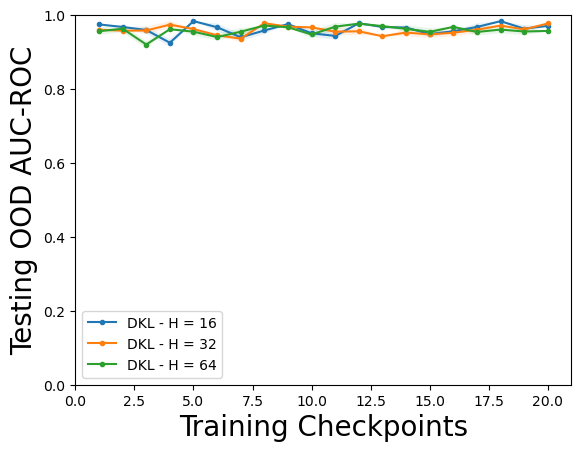
\includegraphics[width=\textwidth]{sections/011_icml2022/resources/CartPoleOOD-v0-AUC-ROC-epistemic_-testing-hyperparameter-latent_dim-dkl.png}
    \end{subfigure}
    \begin{subfigure}{.24\textwidth}
        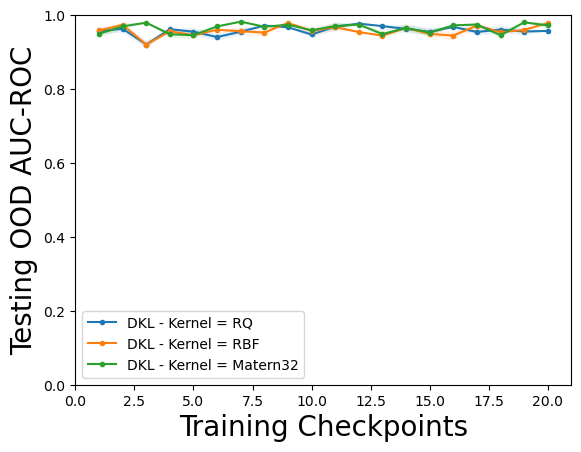
\includegraphics[width=\textwidth]{sections/011_icml2022/resources/CartPoleOOD-v0-AUC-ROC-epistemic_-testing-hyperparameter-kernel-dkl.png}
    \end{subfigure}
        \begin{subfigure}{.24\textwidth}
        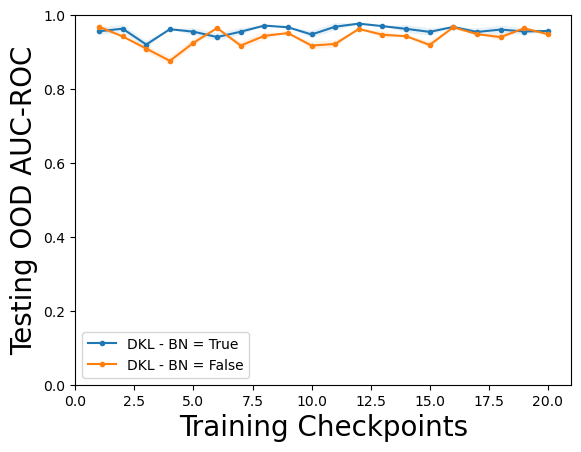
\includegraphics[width=\textwidth]{sections/011_icml2022/resources/CartPoleOOD-v0-AUC-ROC-epistemic_-testing-hyperparameter-bn-dkl.png}
    \end{subfigure}        
    \vspace{-3mm}
    \caption{Hyper-parameter study for DKL w.r.t. the number of inducing points $n$, the latent dimension $H$, the kernel type and the batch norm layer. Ideally, an uncertainty aware-model should achieve high reward and high OOD detection scores.}
    \label{fig:hyperparameter-dkl-cartpole}
    \vspace{-4mm}
\end{figure}